\documentclass[12pt]{article}

\usepackage[
  a4paper, 
  %showframe,
  total={180mm, 240mm}
  ]{geometry}

\usepackage{avant}
\renewcommand*\familydefault{\sfdefault}

\usepackage[T1]{fontenc}
\usepackage[utf8]{inputenc}

\usepackage{tikz}
\usetikzlibrary{calc,arrows.meta,bending,positioning,intersections,through}

\usepackage{xcolor}

\definecolor{bg0}{HTML}{FFFBEF}
\definecolor{bg1}{HTML}{F8F5E4}
\definecolor{bg2}{HTML}{F2EFDF}

\definecolor{red}{HTML}{F85552}
\definecolor{orange}{HTML}{F57D26}
\definecolor{green}{HTML}{8DA101}
\definecolor{yellow}{HTML}{DFA000}
\definecolor{blue}{HTML}{3A94C5}
\definecolor{aqua}{HTML}{35A77C}
\definecolor{purple}{HTML}{DF69BA}

\definecolor{green_light}{HTML}{93B259}
\definecolor{red_light}{HTML}{E66868}

\definecolor{fg}{HTML}{5C6A72}

\color{fg}
\pagecolor{bg0}

\newcommand{\drawline}[2]{
  \fill[aqua!80] ($#1+(2.2, 0)$) circle (2pt);
  \fill[aqua!80] ($#2-(2.2, 0)$) circle (2pt);
}

\title{Bazy danych projekt}
\author{Weronika Jakimowicz}
\date{13.06.2024}

\usepackage{listings}

\lstset{ 
  frame=L,
  backgroundcolor=\color{bg1},
  basicstyle=\large\ttfamily, 
  breaklines=true, 
  morekeywords={article, points, institution, author, open, newuser, deluser},
  keywordstyle=\color{orange}
}

\def\inline{\lstinline[basicstyle=\ttfamily\large\color{orange!50!fg}]}

\makeatletter
\renewcommand*{\verbatim@font}{\ttfamily\large\color{orange!50!fg}}
\makeatother

\begin{document}
\maketitle 

\section{Dokumentacja}

\begin{lstlisting}
open <host> <baza> <login> <password>
\end{lstlisting}

Otwiera połączenie z \inline{<baza>} jako użytkownik \inline{<login>} o haśle \inline{<password>}. Jeśli połączenie powiodło się, zwraca \inline{"status": "OK"}, wpp. dostaniemy \inline{"status": "ERROR"}

\begin{lstlisting}
newuser <secret> <newlogin> <newpassword>
\end{lstlisting}

Dodaje nowego użytkownika aplikacji

\begin{lstlisting}
article <login> <password> <date> <title> <conference> <author_list> 
\end{lstlisting}

Pozwala dodawać nowe papery do bazy danych. Jeśli wartość \inline{<conference>} nie jest identyfikatorem istniejącej już w bazie \inline{conferences} konferencji, to dodajemy ją i ustawiamy punkty od daty publikacji paperu na $0$. %Jeśli próbujemy dodać paper z nieistniejącej konferencji, program zwróci \inline{"status": "ERROR"}.

W przypadku dodawania paperów, instytucja jak i autor zostaną dodani jeśli jeszcze nie istnieli, a w przypadku zmiany afiliacji autora, zostanie to odnotowane w odpowiedniej tabeli.

\begin{lstlisting}
points <login> <password> <date> <points_list>
\end{lstlisting}

Dla każdej konferencji \inline{<conference_id>} podanej na liście \inline{<points_list>=[<conference_id>, <points>]} ustawia punkty na \inline{<points>} dla wszystkich prac napisanych po dacie \inline{<date>}.

\begin{lstlisting}
institution <start_date> <end_date>

author <start_date> <end_date>
\end{lstlisting}

Zwraca listę instytucji/autorów wraz ze zdobytą przez nich ilością punktów między \inline{<start_date>} a \inline{<end_date>}. Jeśli instytucja/autor nie zdobyła w tym okresie żadnych punktów, to nie zostaje wypisana.

\newpage

\section{Model konceptualny}

\textbf{Legenda:}
\begin{itemize}
  \item strzałki oznaczają \emph{foreign key}
  \item pogrubiony czerwony tekst i ciemniejsze tło to \emph{primary key}
  \item elementy z własnością \inline{NOT NULL} są oznaczone $\neq\emptyset$.
\end{itemize}
Dodatkowo, wartość pola \inline{secret} w tabeli \inline{user logins} zawsze musi wynosić 

\inline{'d8512346fbc5bb7a325ca4'}


\begin{center}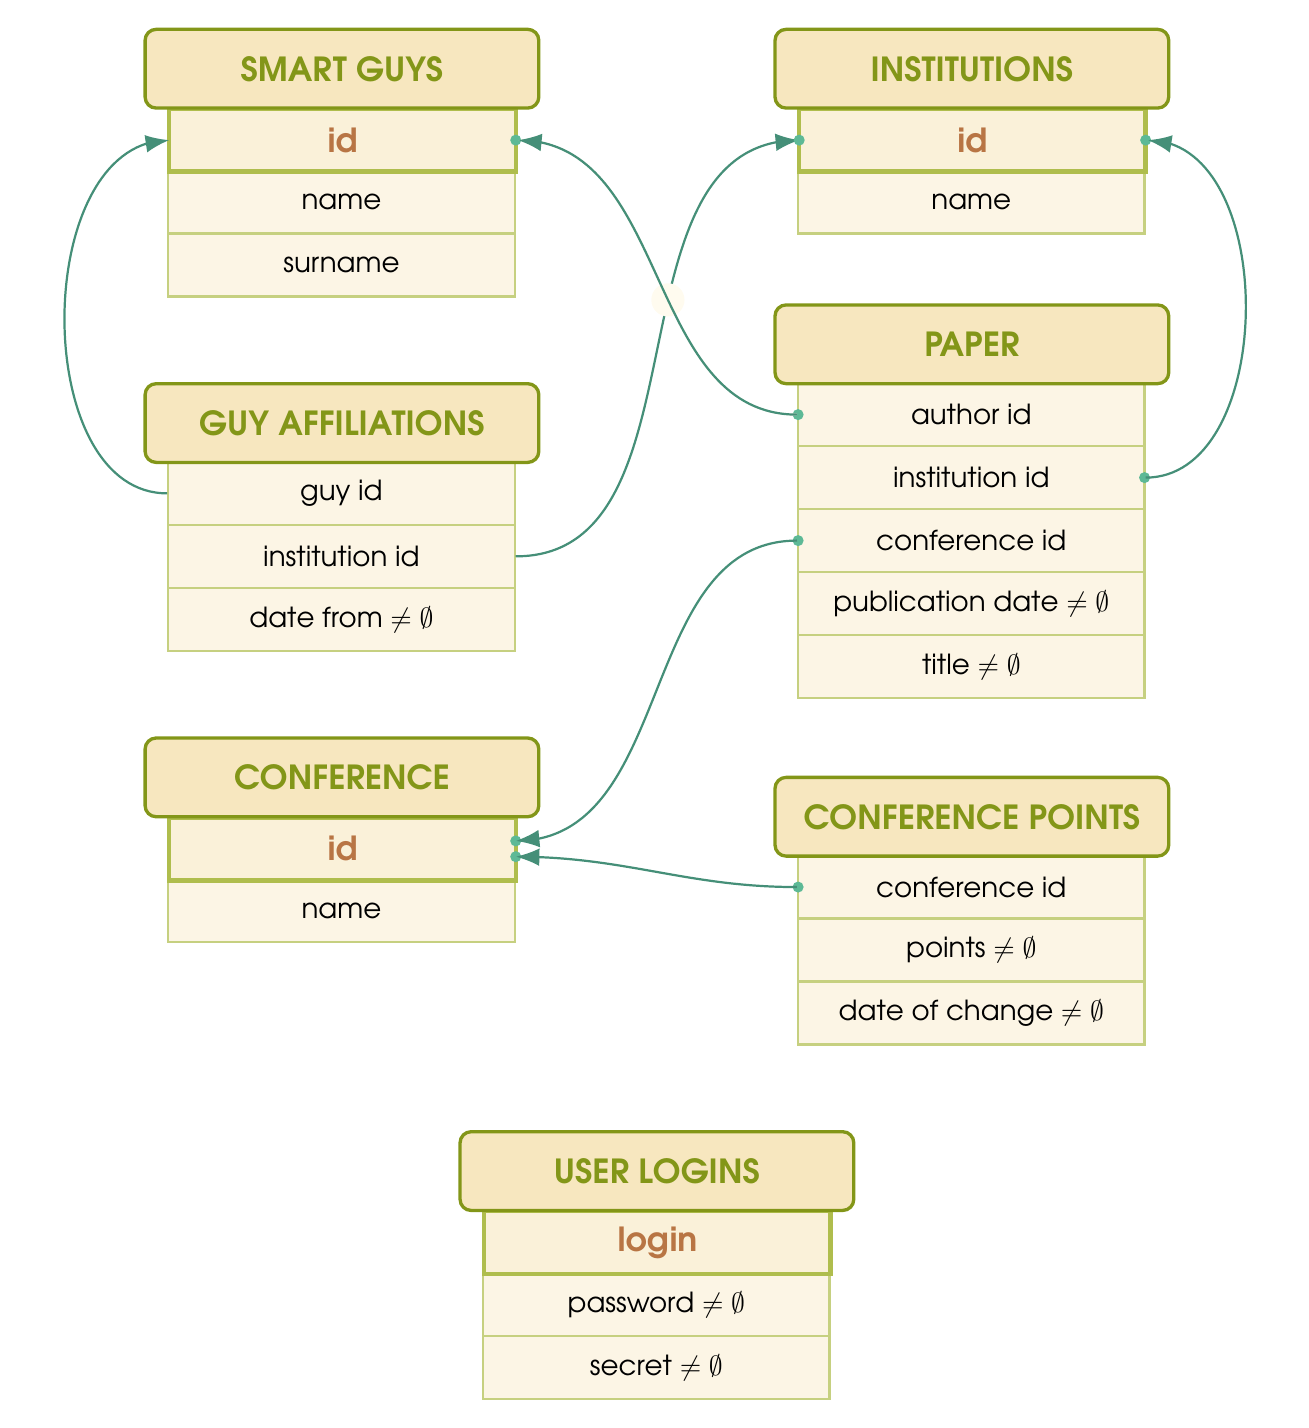
\begin{tikzpicture}[ 
  titlenode/.style={
    rectangle,
    very thick,
    draw=green!80!fg, 
    fill=yellow!25, 
    rounded corners, 
    minimum width=5cm, 
    minimum height=10mm, 
    font=\color{green!80!fg}\bfseries\large
  }, 
  bodynode/.style={
    rectangle, 
    draw=green!50,
    fill=yellow!10,
    thick,
    minimum width=4.4cm, 
    minimum height=8mm
  },
  primkey/.style={
    rectangle, 
    draw=green!70,
    fill=yellow!15,
    ultra thick,
    minimum width=4.4cm, 
    minimum height=8mm, 
    font=\bfseries\color{orange!60!fg}\large
  }
  ]

  % smart guys
  \begin{scope}
    % \node[anchor=north west, bodynode] (smart-aff-id) at (0.3, -1-.8*1) {institution id};
    \node[anchor=north west, bodynode] (smart-name) at (0.3, -1-.8) {name};
    \node[anchor=north west, bodynode] (smart-surname) at (0.3, -1-.8*2) {surname};
    \node[anchor=north west, primkey] (smart-id) at (0.3, -1) {id};

    \node[anchor=north west, titlenode] (smart-title) at (0,0) {SMART GUYS};
  \end{scope}
  
  \begin{scope}
    \node[anchor=north west, bodynode] (inst-name) at (8.3, -1-.8) {name};
    \node[anchor=north west, primkey] (inst-id) at (8.3, -1) {id};

    \node[anchor=north west, titlenode] (inst-title) at (8,0) {INSTITUTIONS};
  \end{scope}  

  % paper
  \begin{scope}[shift={(0,-.5)}]
    \node[anchor=north west, bodynode] (paper-auth-id) at (8.3, -4) {author id};
    \node[anchor=north west, bodynode] (paper-inst-id) at (8.3, -4-.8) {institution id};
    \node[anchor=north west, bodynode] (paper-conf-id) at (8.3, -4-2*.8) {conference id};
    \node[anchor=north west, bodynode] (paper-date) at (8.3, -4-3*.8) {publication date $\neq\emptyset$};
    \node[anchor=north west, bodynode] (paper-tit) at (8.3, -4-4*.8) {title $\neq\emptyset$};
      
    \node[anchor=north west, titlenode] (paper-title) at (8,-3) {PAPER};
  \end{scope}
  
  % conference
  \begin{scope}[shift={(0, -3.5)}]
    \node[anchor=north west, bodynode] (conf-name) at (.3, -6.5-.8) {name};
    % \node[anchor=north west, bodynode] (conf-pkt) at (.3, -6.5-2*.8) {current points};
    \node[anchor=north west, primkey] (conf-id) at (.3, -6.5) {id};
  
    \node[anchor=north west, titlenode] (conf-title) at (0,-5.5) {CONFERENCE};
  \end{scope}
   
  % conference points
  \begin{scope}
    \node[anchor=north west, bodynode] (conf-pkt-id) at (8.3, -9.5-1) {conference id};
    \node[anchor=north west, bodynode] (conf-pkt-pkt) at (8.3, -10.5-.8) {points $\neq\emptyset$};
    \node[anchor=north west, bodynode] (conf-pkt-date) at (8.3, -10.5-2*.8) {date of change $\neq\emptyset$};
  
    \node[anchor=north west, titlenode] (conf-pkt-title) at (8,-9.5) {CONFERENCE POINTS};

  \end{scope}
  
  % guy affiliation
  \begin{scope}[shift={(0,1)}]
    \node[anchor=north west, bodynode] (guy-id) at (.3, -6.5) {guy id};
    \node[anchor=north west, bodynode] (aff-inst-id) at (.3, -6.5-.8) {institution id};
    \node[anchor=north west, bodynode] (aff-date) at (.3, -6.5-2*.8) {date from $\neq\emptyset$};
      
    \node[anchor=north west, titlenode] (aff-title) at (0,-5.5) {GUY AFFILIATIONS};
  \end{scope}



  %\drawline{(smart-aff-id)}{(inst-id)}
  \drawline{($(conf-id)+(2.2, .1)$}{(conf-pkt-id)}
  \drawline{(smart-id)}{(paper-auth-id)}
  \fill[aqua!80] ($(conf-id)+(2.2, -.1)$) circle (2pt);
  \fill[aqua!80] ($(paper-conf-id)+(-2.2, 0)$) circle (2pt);
  
  \fill[aqua!80] ($(inst-id)+(2.2, 0)$) circle (2pt);
  \fill[aqua!80] ($(paper-inst-id)+(2.2, 0)$) circle (2pt);
  
  \draw[thick, aqua!60!fg, -{Latex[length=3mm]}, name path=AFF-INST] (aff-inst-id) to[out=0, in=180] ($(inst-id)+(-2.2, 0)$);
  \fill [aqua!80] ($(inst-id) + (-2.2, 0)$) circle (2pt);

  \draw[thick, aqua!60!fg, -{Latex[length=3mm]}] (guy-id) to[out=180, in=180] ($(smart-id)+(-2.2, 0)$);
  \draw[thick, aqua!60!fg, -{Latex[length=3mm]}] (paper-inst-id) to[out=0, in=0] (inst-id);
  
  \draw[thick, bg0, -{Latex[length=3mm]}, name path=SMART-INST] (paper-auth-id) to[out=180, in=0] (smart-id);
  \path [name intersections={of=AFF-INST and SMART-INST,by=E}];
  \node (inters) at (E) {};
  \fill[bg0] (inters) circle (6pt);
  \draw[thick, aqua!60!fg, -{Latex[length=3mm]}, name path=SMART-INST] (paper-auth-id) to[out=180, in=0] (smart-id);
  \draw[thick, aqua!60!fg, -{Latex[length=3mm]}] (paper-conf-id) to[out=180, in=0] ($(conf-id)+(2.2, .1)$);
  \draw[thick, aqua!60!fg, -{Latex[length=3mm]}] (conf-pkt-id) to[out=180, in=0] ($(conf-id)+(2.2, -0.1)$);

  
  \begin{scope}[shift={(4,-8.5)}]
    \node[anchor=north west, bodynode] (aff-inst-id) at (.3, -6.5-.8) {password $\neq\emptyset$};
    \node[anchor=north west, bodynode] (aff-date) at (.3, -6.5-2*.8) {secret $\neq\emptyset$};
    
    \node[anchor=north west, primkey] (guy-id) at (.3, -6.5) {login};
      
    \node[anchor=north west, titlenode] (aff-title) at (0,-5.5) {USER LOGINS};
  \end{scope}

\end{tikzpicture}\end{center}

% W powyższym diagramie strzałki oznaczają foreign keys, natomiast primary key jest oznaczony czerwonym tesktem, pogrubioną ramką i ciemniejszym tłem. Pola, które nie mogą być puste mają dopisane $\neq\emptyset$.

\end{document}
